\documentclass{article}
\usepackage[utf8]{inputenc}
\usepackage{proof}
\usepackage{amsmath,amssymb, color, tikz}
\usepackage{fullpage}
\usepackage[pdf]{pstricks}
\usepackage[ruled,vlined,linesnumbered]{algorithm2e}
\usepackage{algorithmic}
\usepackage{todonotes}
\usepackage[hidelinks]{hyperref}
\usepackage{cleveref}
\usepackage{stmaryrd}
\usepackage{booktabs}
\usepackage{float}
% \usepackage{thmtools} 
\usepackage{thm-restate}

\usepackage{graphicx}
\graphicspath{ {./images/} }

\newcommand{\haitian}[1]{\textcolor{teal}{Haitian: #1}}
\newcommand{\malvin}[1]{\textcolor{blue}{Malvin: #1}}
\newcommand{\avijeet}[1]{\textcolor{olive}{Avijeet: #1}}
\usepackage[
    backend=biber,
    style=alphabetic,
    natbib=true,
    url=true,
    maxcitenames=3,
    maxbibnames=9,
    abbreviate=false,
    eprint=false,
    doi=true
]{biblatex}
\DeclareFieldFormat{url}{\url{#1}}
\DeclareFieldFormat{doi}{\url{https://doi.org/#1}}
\addbibresource{refs.bib}

\newcommand{\Decide}{\mathsf{Decide}}
\newcommand{\DecidePSPACE}{\mathsf{DecidePSPACE}}
\newcommand{\PSPACEReach}{\mathsf{PSPACEReach}}
\newcommand{\CreateDelta}{\mathsf{CreateDelta}}
\newcommand{\StringRepresent}{\mathsf{StringRepresent}}
\newcommand{\StoreStrings}{\mathsf{StoreStrings}}
\newcommand{\ResidueByLetter}{\mathsf{ResidueByLetter}}
\newcommand{\ResidueByWord}{\mathsf{ResidueByWord}}
\newcommand{\AuxOut}{\mathsf{AuxOut}}
\newcommand{\Residue}{\mathsf{Residue}}
\newcommand{\GetSet}{\mathsf{GetSet}}
\newcommand{\TRUE}{$\mathsf{TRUE}$ }
\newcommand{\NO}{$\mathsf{FALSE}$ }

\newcommand\ldiaarg[1]{\langle#1\rangle}

\newcommand{\cA}{\mathcal{A}}
\newcommand{\cB}{\mathcal{B}}
\newcommand{\cC}{\mathcal{C}}
\newcommand{\cD}{\mathcal{D}}
\newcommand{\cE}{\mathcal{E}}
\newcommand{\cF}{\mathcal{F}}
\newcommand{\cG}{\mathcal{G}}
\newcommand{\cH}{\mathcal{H}}
\newcommand{\cI}{\mathcal{I}}
\newcommand{\cJ}{\mathcal{J}}
\newcommand{\cK}{\mathcal{K}}
\newcommand{\LL}{\mathcal{L}}
\newcommand{\M}{\mathcal{M}}
\newcommand{\cN}{\mathcal{N}}
\newcommand{\cO}{\mathcal{O}}
\newcommand{\cP}{\mathcal{P}}
\newcommand{\cQ}{\mathcal{Q}}
\newcommand{\cR}{\mathcal{R}}
\newcommand{\cS}{\mathcal{S}}
\newcommand{\cT}{\mathcal{T}}
\newcommand{\cU}{\mathcal{U}}
\newcommand{\cV}{\mathcal{V}}
\newcommand{\cW}{\mathcal{W}}
\newcommand{\cX}{\mathcal{X}}
\newcommand{\cY}{\mathcal{Y}}
\newcommand{\cZ}{\mathcal{Z}}

\newcommand{\hatK}{\widehat{K}}

\newcommand{\POL}{\mathsf{POL}}
\newcommand{\pPOL}{\mathsf{P-POL}}
\newcommand{\PAL}{\mathsf{PAL}}
\newcommand{\DEL}{\mathsf{DEL}}
\newcommand{\Ag}{\mathsf{I}}

\newcommand{\EPL}{\mathsf{EPL}}
\newcommand{\reach}{\mathsf{PSPACEReach}}
\newcommand{\GetSetNP}{\mathsf{GetSetNP}}
\newcommand{\Tr}{\mathsf{true}}
\newcommand{\Fa}{\mathsf{false}}
\newcommand{\tr}{\mathsf{tr}}
\newcommand{\starfree}{\mathsf{Star\mbox{-}Free}}
\newcommand{\word}{\mathsf{Word}}
\newcommand{\wPOLn}{\mathsf{wPOL_n}}
\newcommand{\existential}{\mathsf{Existential}}
\newcommand{\PSPACE}{\mathsf{PSPACE}}
\newcommand{\NPSPACE}{\mathsf{NPSPACE}}
\newcommand{\PTime}{\mathsf{P}}
\newcommand{\NP}{\mathsf{NP}}
\newcommand{\PTIME}{\mathsf{PTIME}}
\newcommand{\automaton}{\mathcal A}
\newcommand{\modelM}{\mathcal M}
\newcommand{\languageof}[1]{L({#1})}
\newcommand{\set}[1]{\{#1\}}
\newcommand{\suchthat}{\mid}
\newcommand{\union}{\cup}
\newcommand{\Union}{\bigcup}
\newcommand{\regdiv}{\ensuremath{\backslash}}

\newcommand{\outof}{\mathsf{outof}}
\newcommand{\goto}{\mathsf{goto}}
\newcommand{\change}{\mathsf{change}}

\DeclareMathOperator*{\bigsem}{;}

\newtheorem{theorem}{Theorem}[section]
\newtheorem{proposition}[theorem]{Proposition}
\newtheorem{corollary}[theorem]{Corollary}
\newtheorem{remark}[theorem]{Remark}
\newtheorem{lemma}[theorem]{Lemma}
\newtheorem{claim}[theorem]{Claim}
\newtheorem{definition}[theorem]{Definition}
\newtheorem{question}[theorem]{Question}
\newtheorem{example}[theorem]{Example}
\newtheorem{conjecture}[theorem]{Conjecture}
\newtheorem{observation}[theorem]{Observation}
\newtheorem{note}[theorem]{Note}
\newtheorem{notation}[theorem]{Notation}

% Two part definition
\newcommand{\twopartdef}[4]{
  \left\{
    \begin{array}{ll}
      #1 & #2 \\
      #3 & #4
    \end{array}
  \right.
}

\newcommand{\N}{\ensuremath{\mathcal{N}}} % MG: What is this used for?

\newcommand{\F}{\ensuremath{\mathcal{F}}} % knowledge or belief structure
\newcommand{\X}{\ensuremath{\mathcal{X}}} % transformer


% \newcommand{\Tr}{\mathsf{true}}
% \newcommand{\Fa}{\mathsf{false}}
\newcommand{\chk}{\mathsf{check}}
\newcommand{\chkdel}{\mathsf{checkDEL}}
\newcommand{\chkfcdel}{\mathsf{chkfcDEL}}
\newcommand{\chkfcdelK}{\mathsf{checkDELK}}
\renewcommand{\phi}{\varphi}

\tikzstyle{rectNode} = [rectangle, text centered, draw = black]
\tikzstyle{fastate} = [circle, text centered, draw = black]
\tikzstyle{dots} = [circle, draw = black, fill = black, inner sep=1pt]


\title{Logic for Planning by Goal Recognition}
\author{}

\begin{document}

\maketitle


\section{Working Example}
Consider two robots $1, 2$ in a warehouse. There are three rooms in the warehouse $A, B, C$, all of them attached to a common hall. One can only enter every other room via the common hall. 

Initially, both the robots are in room $C$ with two boxes $B_1, B_2$ in the same room. The goal is to either put both the boxes in room $A$ or $B$.

\section{Modelling}
\begin{definition}
    The static knowledge model is based on the usual Kripke model. Let us call it the goal model $\M = \ldiaarg{W, \{\sim_i\}_{i\in\Ag}, V, Exp}$ such that:
    \begin{itemize}
        \item $W$ is the set of possible worlds
        \item $\sim_i$ is the indistinguishability of agents among goals
        \item $V: W\rightarrow 2^\cP$ is the propositional valuation of the possible worlds.
        \item $Exp: W\times \Ag\rightarrow Reg_{\Sigma}$ is the private expectation. $Exp(w, i)$ is a regular expression interpreting what $i$ expects to observe.
    \end{itemize}
\end{definition}
% We consider the following knowledge model of the example in section 1. 
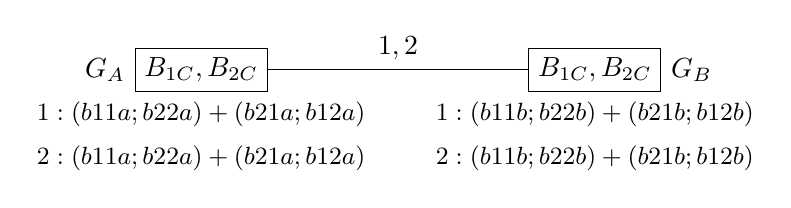
\begin{tikzpicture}
    \centering
    \node[rectNode] (g1) {$B_{1C}, B_{2C}$};
    \node[rectNode] (g2) at (5, 0) {$B_{1C}, B_{2C}$};

    \node[left = 0mm of g1] {$G_A$};
    \node[right = 0mm of g2] {$G_B$};
    \node[below = 0mm of g1] (fexp) {\small$1: (b11a;b22a) + (b21a;b12a)$};
    \node[below = 0mm of fexp] {\small$2: (b11a;b22a) + (b21a;b12a)$};
    \node[below = 0mm of g2] (fexp2) {\small$1: (b11b;b22b) + (b21b;b12b)$};
    \node[below = 0mm of fexp2] {\small$2: (b11b;b22b) + (b21b;b12b)$};

    \draw (g1) edge node[above] {$1, 2$} (g2);
\end{tikzpicture}
\subsection{Action model}
\begin{definition}
    The action model is also based on the usual DEL-like action models. Here $\Sigma$ is the list of all events.
    \begin{itemize}
        \item $\Sigma$ finite set of all events.
        \item $\sim_i\subseteq\Sigma$ is the indistinguishability relation of agent $i$.
        \item $pre:\Sigma\rightarrow\LL_K$ is the precondition formula for each event.
        \item $post:\Sigma\times\cP\rightarrow\{\top,\bot\}$ is the post-condition.
    \end{itemize}
\end{definition}
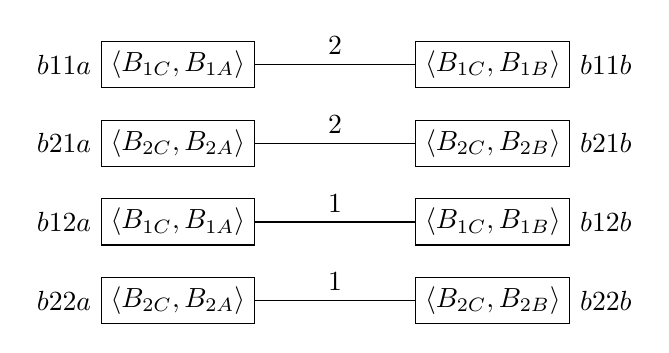
\begin{tikzpicture}
    \node[rectNode] (b11a) {$\ldiaarg{B_{1C}, B_{1A}}$};
    \node[rectNode] (b11b) at (4,0) {$\ldiaarg{B_{1C}, B_{1B}}$};
    \node[left = 0mm of b11a] {$b11a$};
    \node[right = 0mm of b11b] {$b11b$};

    \node[rectNode] (b21a) at (0,-1) {$\ldiaarg{B_{2C}, B_{2A}}$};
    \node[rectNode] (b21b) at (4,-1) {$\ldiaarg{B_{2C}, B_{2B}}$};
    \node[left = 0mm of b21a] {$b21a$};
    \node[right = 0mm of b21b] {$b21b$};

    \node[rectNode] (b12a) at (0,-2) {$\ldiaarg{B_{1C}, B_{1A}}$};
    \node[rectNode] (b12b) at (4,-2) {$\ldiaarg{B_{1C}, B_{1B}}$};
    \node[left = 0mm of b12a] {$b12a$};
    \node[right = 0mm of b12b] {$b12b$};

    \node[rectNode] (b22a) at (0,-3){$\ldiaarg{B_{2C}, B_{2A}}$};
    \node[rectNode] (b22b) at (4,-3) {$\ldiaarg{B_{2C}, B_{2B}}$};
    \node[left = 0mm of b22a] {$b22a$};
    \node[right = 0mm of b22b] {$b22b$};


    \draw (b11a) edge node[above] {$2$} (b11b);
    \draw (b21a) edge node[above] {$2$} (b21b);
    \draw (b12a) edge node[above] {$1$} (b12b);
    \draw (b22a) edge node[above] {$1$} (b22b);
\end{tikzpicture}
\end{document}


